% Adapted from the TeX Live PGFPlots groupplots manual, section 5.8.
\documentclass[border=2pt]{standalone}
\usepackage{pgfplots}
\usepgfplotslibrary{groupplots}

\begin{document}
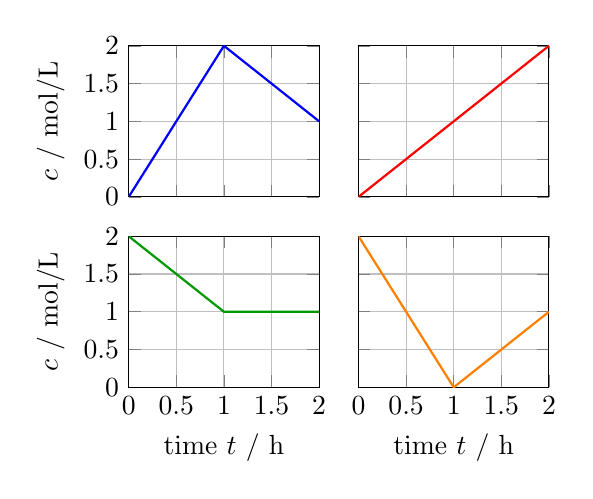
\begin{tikzpicture}
\begin{groupplot}[
  group style={
    group name=measurements,
    group size=2 by 2,
    x descriptions at=edge bottom,
    y descriptions at=edge left,
    horizontal sep=0.5cm,
    vertical sep=0.5cm
  },
  width=4cm,
  height=3.5cm,
  xmin=0, xmax=2,
  ymin=0, ymax=2,
  xlabel={time $t$ / h},
  ylabel={$c$ / mol/L},
  grid=major
]
  \nextgroupplot
    \addplot[blue, thick] coordinates {(0,0) (1,2) (2,1)};
  \nextgroupplot
    \addplot[red, thick] coordinates {(0,0) (1,1) (2,2)};
  \nextgroupplot
    \addplot[green!60!black, thick] coordinates {(0,2) (1,1) (2,1)};
  \nextgroupplot
    \addplot[orange, thick] coordinates {(0,2) (1,0) (2,1)};
\end{groupplot}
\end{tikzpicture}
\end{document}
